\documentclass{scrartcl}
\usepackage{amsmath, amssymb, amsthm}
\usepackage[british]{babel}
\usepackage[utf8]{inputenc}

\usepackage{lmodern}
\usepackage[T1]{fontenc}
\usepackage[babel=true]{microtype}

\usepackage{geometry}
\usepackage{color}
\usepackage{graphicx}
\usepackage{hyperref}
\usepackage{listings}
\usepackage{graphicx}
\graphicspath{ {images/} }

\newcommand{\todo}[1] {{\color{red}(TODO: #1)}}



\begin{document}


\title{Servo}
\subtitle{An Analysis for "Testen, Verifizieren und Analysieren von Software", Winter Term 2015/16, Hasso-Plattner-Institute}
\author{Johannes Linke, David Schumann}
\maketitle


\section{About the Project}

The current generation of web browsers (Internet Explorer, Chrome, Firefox, and Safari) are mostly built on old and large code bases, and important design decisions whose results are visible still today have been made in a time where the IT landscape looked vastly different in terms of hardware, end-user device form factors, and security.

The Servo project aims at building a new browser engine for today's requirements. It is designed to be highly parallel, leveraging multi-core hardware and saving power on mobile devices, and exceptionally secure, by using a new programming language that eliminates certain classes of security-relevant programming errors.

The Servo project is developed and maintained by Mozilla Research in cooperation with Samsung. It is one of the largest projects being written in the Rust programming language, which is developed as well by Mozilla Research. We are learning Rust in our free time and wanted to test one of the major projects using it.


\subsection{Main Programming Language: Rust}

While some dependencies and build infrastructure code are written in different languages, the main programming language remains Rust. This works well with the main focus of Servo: a highly parallel, safe and fast alternative to current engines. Rust was designed to be just that: For instance, it is memory safe by design and requires the programmer to be very explicit with typing and error handling. This helps catching most errors at compilation time using static analysis. More details about the features of the Rust language are explained in section \ref{rust_features}.


\subsection{Requirements, Specifications and Documentation}
\todo{this headline?}

Servo is an open source project hosted on GitHub\footnote{\url{https://github.com/servo/servo}}. As with most open source projects, the core developers have established a well documented GitHub workflow\footnote{\url{https://github.com/servo/servo/wiki/Github-workflow}}. It consists of the standard steps that go with any Github project where you don't have write access:
\begin{enumerate}
    \item Fork the original repository
    \item Write and commit your contribution into a branch in your fork.
    \item Open a Pull Request from the branch in your repository to the original one
    \item Discuss and fix any questions and suggestions by the reviewer.
    \item The reviewer states his approval, triggers build bot to run automated tests and merges the Pull Request
\end{enumerate}

Every Pull Request needs to pass the contribution checklist\footnote{\label{contributing}\url{https://github.com/servo/servo/blob/master/CONTRIBUTING.md}}. It covers technicalities such as: Every change needs to be accompanied by ``tests relevant to the fixed bug or new feature''\footnote{See last point at footnote \ref{contributing}.} which is to be evaluated by one of the reviewers from the core team, but it also includes the Rust Code of Conduct\footnote{\url{http://www.rust-lang.org/conduct.html}} to ensure a friendly and welcoming environment for all contributors.  \\

Further documentation can be found in the Servo wiki\footnote{\url{https://github.com/servo/servo/wiki}} hosted on Github. In addition to the above points it includes protocol notes on the biweekly meetings, long and short term goals, and a vast amount of documents aimed at helping with development and testing.


\subsection{Current Testing Status} \label{test_status}

As of January 2016 the code base of Servo core (without dependencies) contains 110k lines of code. These are tested with over 11,000 tests that are run using different commands:
\begin{itemize}
    \item \textbf{./mach test-unit}: Runs 233 low level test binaries, that test important code. Especially used in dependencies.
    \item \textbf{./mach test-wpt}: Runs 3764 web-platform-tests. 
    \item \textbf{./mach test-css}: Runs 7097 CSS Working Group tests.
    \item \textbf{./mach test-ref}: Runs 5 reference tests (including the famous acid2 test\footnote{\url{http://www.webstandards.org/files/acid2/test.html}}). These consist of rendering two pages and comparing them.
    \item \textbf{./mach test-dromaeo}: Runs the Dromaeo test suite. This suite is geared towards javascript performance testing. It did not execute successfully when we called it.
    \item \textbf{./mach test-jquery}: Runs the jQuery test suite. It did not execute successfully when we called it.
    \item \textbf{./mach test-tidy}: Runs the source code tidiness check.
\end{itemize}

Some other commands are still documented in the wiki and help pages but are now deprecated (like ./mach test-content). These tests currently contain about 70-80 tests that fail intermittently. This often slows down the process of contributing working code. We encountered this while sending a Pull Request that fixed about 130 code lints found by rust-clippy (see chapter \ref{clippy}).

\paragraph{Tracking and Fixing of Issues}
As with most open source projects hosted on Github, the issue tracker\footnote{\url{https://github.com/features}} is used to track bugs, issues and features. It employs several handy features that make it easy to organize the frequent discussions and comments surrounding Issues and Pull Request. Both get assigned numbers, which when mentioned in any comment automatically link to the corresponding Issue or Pull Request. Issues automatically record when they were ``mentioned'' in another discussion. This builds a coherent map of Issues and their corresponding fixes (WIP or not).

\paragraph{Mozilla's ``mach'' System}
Mozilla's build system ``mach'' (from the german word ``machen'': to do) is at the core of the Servo project. Besides providing commands for running the various test suites as introduced earlier, it also makes it easy to compile and run the Servo binary or other related tools like rust-clippy (see chapter \ref{clippy}). While the Rust compiler brings its own package manager ``cargo'', which can also be used for compiling projects and running tests, it is not powerful enough (yet) to fulfill all the requirements a large project like Servo has, and thus its commands were wrapped inside mach.


\subsection{Servo's Roadmap}
Short-term goals of the Servo project are Windows support, finishing WebRender, a GPU-based rendering engine, and adding a GUI to Servo, whose window currently consists solely of the rendered output without GUI controls.
 
Being a research project, Servo's long-term outcomes are rather open-ended, but preliminary performance testing shows major advantages over Gecko, the engine of Firefox, besides the security improvements that come naturally with choosing Rust and large architectural improvements made possible by the clean-slate approach. Replacing Gecko with Servo in Mozilla's Firefox products appears like a reasonable goal, albeit the project is years away from implementing all of Gecko's functionality. As a compromise, Mozilla plans to use smaller, isolated modules written for Servo in Gecko, and will evaluate the feasibility of a standalone Servo browser, most likely starting with the Android platform.




\section{Initial Test Plan}


\subsection{The five V\&V questions}
\todo{well...}

\paragraph{When do verification and validation start? When are they complete?}
V \& V starts with the begining of the project. As with many open source project that are developed by the community, the stakeholder or ``customer'' is the community itself. Which means that developer and customer are often the same person. In the case of Servo the software is validated in bi-weekly meetings\footnote{\url{https://github.com/servo/servo/wiki/Meetings}} where both short-term next steps and long term milestones are discussed.\\
  
  Verification is done through an extensive testing system. It is maintained by every developer as every code change needs to be accompanied by a test before it is merged into the code base. This test suite runs on every reviewed pull request, via two build servers (bors-servo\footnote{\url{https://github.com/bors-servo}} and buildbot\footnote{\url{http://servo-buildbot.pub.build.mozilla.org/}}). This ensures that no new bugs are introduced into the system.\\
  
V \& V will never be complete. Even after the release there will always be bog fixes or new features that need to be tested as well. One could argue that V \& V ends when the project gets abandoned but you can hardly call that a complete state.

\paragraph{What particular techniques should be applied during development?}
Servo is already a well tested system. But it lacks a lot of even basic V \& V features like a report on any kind of test coverage. Furthermore we would like to see tests about parallel execution. These are hard to write and execute but a project having concurrency as one of it's main three points should test it.

\paragraph{How can we assess the readiness of a product?} 
The readiness of the product is currently assessed in biweekly meetings of the Servo core team. There should be assessment by an outside party to prevent building unneccessary features and to keep a fresh new perspective regarding V \& V on the project.

\paragraph{How can we control the quality of successive releases?}
The Servo project already has the basic automated testing feature covered: Regression tests with the merge of every Pull Request. This assures, that no change makes the code base worse according to the test suite. Which in turn places the whole quality assurance on software tests. It is important, that these are as complete as possible. In addition to test that test parallel execution, performance tests should also be part of Servos test suite. Benchmarks of Servo vs Gecko were computed at some point\footnote{\url{https://www.phoronix.com/scan.php?page=news_item&px=MTgzNDA}}. But including them in the test suite would help to find less performant changes, that slow execution down from one release to another.

\paragraph{How can the development process itself be improved?}
The development process used by Servo is very standard to many professional open source projects with not exorbitant budgets. When you don't have the resources to hire a separate testing team or a V \& V specialist the approach to have every developer test his own code and do full regression testing at every step is a successful model. It is hard to improve it without raising the budget. 


\subsection{Test Classifications}

\paragraph{Validation and Defect Testing}
The biggest part of the test suite used in the Servo project is focused on validation testing. The whole web platform test (WPT) suite and CSS WG suite are geared to validate that all aspects and features of html, css and javascript are implemented. The few reference tests contain defect tests such as the famous acid2 test. Here a lot of different html and css rules are used to draw a smiley. If any of those rules are not implemented correctly, the smiley will not be drawn correctly.

\begin{figure}[h]
    \centering
    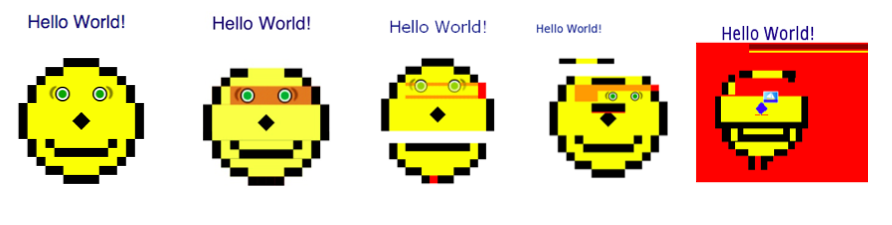
\includegraphics[width=\textwidth]{acid2}
    \caption{Acid2. Correct rendering on the left. All others show rendering flaws}
\end{figure}

\paragraph{Development, Release and User Testing}
\todo{johannes not likes}
These three forms of testing are all present but hardly differentiable in the Servo project. This is due to the fact that the core development team combines developers, release testers and users in the same team. The tests are mostly used during development for regression testing. But there is no separate test suite or separate test team used before releases. It is done by the community but mostly the core members as well. Finally the core developers are also the users, as they represent Mozilla. Ultimately Mozilla wants to replace the gecko\footnote{\url{https://developer.mozilla.org/en-US/docs/Mozilla/Gecko}} engine with Servo. Thus the core team develops, releases and decides when Servo is ready for the user: themselves. From a testers perspective this is not an optimal state to create a complete testing suite. A separate release testing team or at least an internal group posing as the "users" would be helpful to get an outside perspective on the readiness and validity of the product.

\paragraph{Unit-, Integration- and System-testing}
As can be seen in chapter \ref{test_status}, the unit tests only make up a fraction of the overall test suite. Integration tests are sometimes used in the dependencies, but do not get executed when testing the main Servo binary. The biggest part are the system tests. All WPT and CSS WG tests are system level tests as they execute the Servo binary and try to actually use the whole rendering engine by rendering a complete web page, albeit testing only for small sets of features each. This testing approach that focuses mainly on system tests makes sense for testing a web engine, as there are a lot of formal requirements that can easily and exhaustively be tested on the whole product.


\subsection{Consider available artefacts, discuss \& evaluate potentials w.r.t. coverage-based testing for your application}
\todo{do}


\subsection{Develop \& document initial test plan based on your findings}
\todo{do}




\section{Test automation}


\subsection{cargo test}

Rust's package manager cargo already has tools for running tests. Testing is as easy as annotating any method with \texttt{\#[test]}, and then running \texttt{cargo test}. Cargo will then build a testing binary, run all annotated methods and print out a report that looks like this:


\begin{verbatim}
    Compiling gfx_tests v0.0.1 (file:///home/johannes/servo/components/servo)
    Running /home/johannes/servo/target/debug/deps/gfx_tests-9666be7e60be2090

running 6 tests
test text_util::test_transform_compress_none ... ok
test text_util::test_transform_compress_whitespace ... ok
test text_util::test_transform_compress_whitespace_newline_no_incoming ... ok
test text_util::test_transform_compress_whitespace_newline ... ok
test text_util::test_transform_discard_newline ... ok
test font_cache_thread::test_local_web_font ... ok

test result: ok. 6 passed; 0 failed; 0 ignored; 0 measured

\end{verbatim}

Any crashes inside the tests (e.g. by failing assertions) are interpreted as test failures, methods that exit normally are successes.

Cargo's builtin testing features are not meant for large-scale applications and test suites. There are some smaller libraries like stainless \footnote{\url{https://github.com/reem/stainless}} that are extending on cargo's features for example by adding setup and teardown methods, but such libraries haven't seen much use yet. 

Servo uses \texttt{cargo test} for running the unit tests. For running the more complex test suites, it builds the binaries with cargo but uses python scripts to execute the individual tests. See chapter \ref{test_status} for more details.


\subsection{Coverage Tools Using gcov and kcov}

No type of coverage has ever been calculated for the whole Servo project, not even basic statement coverage. As this is one of the most common ways to indicate the completeness of the test suite we looked into creating a test coverage of Servo. We also hoped to find parts in the code base that are not yet covered by tests which we could then further examine. 

\paragraph{gcov}
Gcov\footnote{\url{https://gcc.gnu.org/onlinedocs/gcc/Gcov.html}} is a widely used source code coverage analysis tool that comes with the GNU Compiler Collection (GCC). It is supposed to work with any LLVM-generated files. As the Rust compiler rustc uses LLVM as its backend we tried gcov first to generate a useable test coverage report. Unfortunately, rustc does not yet support all compiler flags that gcov needs to produce coverage data\footnote{Section 4 in \url{http://ltp.sourceforge.net/documentation/technical_papers/gcov-ols2003.pdf}}. This issue has already been reported\footnote{\url{https://github.com/rust-lang/rfcs/issues/646}} but was postponed a year ago due to the 1.0 release of rustc\footnote{\url{https://github.com/rust-lang/rust/issues/690}}. We briefly considered implementing gcov support for rustc which would enable all rust projects to easily generate test coverage reports, but quickly realized that it would be out of scope.

\paragraph{kcov}
The community suggested to try the tool kcov\footnote{\url{https://simonkagstrom.github.io/kcov/}}, which has been used successfully for smaller Rust projects. It works by inserting breakpoints into every line of code and checking them off when they are triggered. This increases execution time significantly but proves to be a robust way to generate code coverage, as it works on arbitrary binaries with debug symbols. Therefore, generating correct debug symbols is enough to let kcov produce a test coverage report. Unfortunately, it does not compile on Mac OS or Windows, so we had to run our tests in a linux (ubuntu) virtual machine which slows down execution even more. Another issue we faced was that the version provided by the package manager (apt-get) was out of date. Compiling kcov from source failed at first, but was quickly fixed by adding another dependency (libbfd-dev) to the build flags.\\

Since Servo relies on mach to prepare the running environment, we couldn't start kcov on the Servo binary directly. Instead, our first coverage report was created by moving the Servo binary to servo\_orig and placing the following script in its place:

\begin{verbatim}

#!/bin/sh
kcov --verify --exclude-pattern=/.cargo,../src /home/joda/servo/cov 
 /home/joda/servo/servo-sync/target/debug/servo_orig "$@"

\end{verbatim}

Now executing \textbf{./mach test} would run our script instead of the Servo binary, which passes all parameters to the original Servo binary but also executes kcov. In theory this should have yielded a complete test coverage report as kcov is also supposed to properly merge several executions of the same binary, which was a necessary feature since mach restarts Servo for each of its tests. Unfortunately every test took 30-60 seconds which implied a whole week of running time to generate a complete coverage report. Also the merging of reports was not working correctly. But as the long execution time already disqualified kcov as a feasible coverage tool we did not continue working on fixing the merging problem.\\

Additionally, the partial coverage reports we got differed from test run to test run. Lines of code covered by one exemplary test ranged from 26976 to 27104 throughout several iterations. These fluctuations are probably caused by non-deterministic behaviour of Servo but could also be caused by inaccurate coverage reports on kcovs side. We can not be completely sure as it would have been infeasible to check the roughly 30,000 lines that were executed in one test run and trace the execution path.


\subsection{Fuzzy Testing Using afl.rs}

afl.rs\footnote{\url{https://github.com/frewsxcv/afl.rs}}, based on American fuzzy lop\footnote{\url{http://lcamtuf.coredump.cx/afl/}}, is a package that allows finding bugs in Rust code through fuzzy testing. It works by taking exemplary input over stdin and mutating it. As a consequence, it requires that the binary to test reads its input over stdin. As Servo does not do this, we looked at Servos html-parser html5ever\footnote{\url{https://github.com/servo/html5ever}} instead. Here we built a test binary that would read html code over stdin and try to parse it. During the setup we realized that afl.rs currently requires quite an old version of Rust (1.2) due to a bug in newer Rust versions\footnote{\url{https://github.com/frewsxcv/afl.rs/issues/11}}. html5ever, however, required Rust 1.4 to work. This problem deemed fuzzy testing the html5ever component or Servo as a whole impossible without extensive debugging of the Rust compiler.




\section{ASA}


\subsection{ASA Features of the Rust Language} \label{rust_features}

Rust has an extensive set of static analysis techniques built-in. They became necessary to achieve the first design goal of the language, safety, while not impeding the second and third, speed and concurrency.

For Servo, these ASA techniques are a crucial part of its security concept. For instance, a large fraction of the security vulnerabilities in Gecko, the engine currently used in Firefox, are related to use-after-free bugs, which are completely eliminated by the Rust compiler.

In the following we describe some of Rust's language concepts that let the Rust compiler prevent certain classes of programming errors that frequently occur in other languages. Finding such errors through static analysis is not always possible in other languages since they are not expressive enough and the programmer can't provide enough information in the code for an ASA tool to perform such an analysis.

\paragraph{Ownership.} In Rust, variables and objects are always ``owned'' by a scope (usually, a block of code delimited by curly braces) or another object. This ownership can be moved, for example by calling a method and handing over the object as a parameter, but the language provides no way to copy the ownership to an object. This way, the owner of an object can be statically determined, and, more importantly, each object can be deleted if its owning object is deleted or the owning scope ends. This way, it can be determined at compile-time when each object has to be deleted, completely eliminating use-after-free bugs, a common source for crashes and security vulnerabilities, and preventing most classes of memory leaks.

\paragraph{Borrowing.} To allow for more flexible movement of data, objects can be temporarily borrowed into other scopes. The compiler statically ensures that there exists either exactly one mutable borrow, through which the object can be mutated, or any number of immutable borrows. By preventing shared mutable state, a lot of programming errors are made impossible, for example data races. A data race occurs if two threads access the same data in an unsynchronized fashion and at least one of them writes. Since there can be only one thread writing at one specific data point at the same time, data races cannot happen. Iterator invalidation is another problem detected at compile time: Since iterating over a container mutably borrows the container, modifying the container, which would need to happen through a second mutable borrow, is not possible.

\paragraph{Safe memory accesses.} Likewise it is not possible to access uninitialized memory and, since pointers are not part of the language, null pointers do not exist as well. Not an ASA technique but related to memory safety are the run-time bounds checks that are mandatory for all Rust data containers.

\paragraph{Code-generating macros.} Rust features a powerful macro syntax. Unlike in C and C++, where macros simply perform text replacements, macros in Rust are hygienic, can generate different code depending on the type of input and take a variable number of parameters among other advantages. In fact, a library has been written that expands regular expressions to native Rust code, enabling a lot of optimization potential as well as compile-time syntax checking on the expression \footnote{\url{https://github.com/rust-lang-nursery/regex}}. Another library enables specifying parsers through a macro-based API \footnote{\url{https://github.com/Geal/nom}}. The resulting parsers are extremely fast and guaranteed to be safe.

\paragraph{Doctests.} As many other languages, Rust defines a syntax to document source code, and as in many other languages, the documentation can contain example code. It might look like this:

\small {
    \begin{verbatim}
    /// Constructs a new `Rc<T>`.
    /// # Examples
    /// ```
    /// use std::rc::Rc;
    /// let five = Rc::new(5);
    /// ```
    pub fn new(value: T) -> Rc<T> {
        // implementation goes here
    }
    \end{verbatim}
}

In Rust, however, these usage examples are executed and tested as part of \texttt{cargo test}. To simplify this process, the example code is automatically completed e.g. with a main function to make it a valid Rust program. More complex examples can be built, e.g. spanning multiple functions, and individual lines can be hidden to focus the user-visible documentation on the relevant parts. The full set of testing facilities, e.g. assertions, is available, making it possible to avoid outdated code examples altogether.

\paragraph{Other features.} There are several smaller features, restrictions and well-chosen defaults of the Rust language that improve the robustness of programs, some of them being ASA techniques: For example, variables are immutable by default, encouraging a less error-prone programming style. Matches (the Rust-equivalent of switch-case statements) must be exhaustive, that is each possible value of the variable that is matched must be handled by a branch, making it impossible for the programmer to forget a case. Integer overflows, being another source of programming errors and security vulnerabilities, make Rust programs crash when compiled in debug mode. And finally, runtime errors such as IO-errors must be explicitly handled by the programmer or will lead to an immediate crash of the program, as opposed to undefined behavior in e.g. C and C++.


\subsection{Lints}

\subsubsection{Lints Reported by the Rust Compiler}

Besides the language features outlined above, the rust compiler has some smaller ASA capabilities in the form of lints which are reported as warnings during compilation. They include unused imports and variables, unnecessarily mutable variables, dead code, variable and function names not following the naming conventions, and unconditional recursions. There are some more lints that are disabled by default like missing documentation of public interfaces and the usage of the \texttt{unsafe} keyword.

\subsubsection{rust-clippy} \label{clippy}

Clippy \footnote{\url{https://github.com/Manishearth/rust-clippy}} is a compiler plugin that expands on the lints shipped with the Rust compiler and checks for common patterns that indicate inefficient, needlessly complex or unidiomatic Rust code. It is exceptionally easy to use since the complete procedure of setting it up consists of adding one line to the cargo configuration and main code file. Having done that, clippy will be run whenever any code in the project is compiled.\\
\\

Example of clippy output:
{
\scriptsize
\begin{verbatim}

servo/components/script/cors.rs:95:9: 98:10 warning: you seem to be trying to use match for destructuring
    a single pattern. Consider using `if let`, #[warn(single_match)] on by default
    
servo/components/script/cors.rs:95         match referer.scheme_data {
servo/components/script/cors.rs:96             SchemeData::Relative(ref mut data) => data.path = vec![],
servo/components/script/cors.rs:97             _ => {}
servo/components/script/cors.rs:98         };

/servo/components/script/cors.rs:95:9: 98:10 help: try
if let SchemeData::Relative(ref mut data) = referer.scheme_data { data.path = vec![] }

for further information visit https://github.com/Manishearth/rust-clippy/wiki#single_match

\end{verbatim}
}

The lints reported by clippy vary in type. Most of them are related to programming style or detecting patterns that were common in old Rust code but can be written simpler in newer versions of Rust. The \texttt{single\_match} lint in the example above is such a lint; the \texttt{if let} construct wasn't available until late 2014. Other lints detect type casts that may lead to loss of precision or truncation, boolean expressions that are tautologies, or obvious bugs like out of bounds accesses with constants. Clippy also includes two lints that warn on complex (as in deeply nested) types and methods with a high cyclomatic complexity.\\
\\
Servo already has clippy integrated, it can be run through \texttt{./mach clippy}. \todo{problems setting up clippy?} Running it, we made the following findings: 
\begin{itemize}
	\item Clippy reported 417 warnings.
    \item Of these, 122 were in autogenerated code.
    \item Another 11 were false positives. Several more might be false positives as well which we haven't investigated further.
    \item The vast majority of lints pointed at code that could be simplified.
    \item Some of these simplifications also led to potentially faster code.
    \item There were eight warnings on complex methods and two warnings on complex types.
    \item Not a single reported lint indicated a possible bug.
\end{itemize}

While working through the warnings, we fixed about 130 of them and made a pull request to Servo \footnote{\url{https://github.com/servo/servo/pull/9123}} and reported several false positives on clippy \footnote{\url{https://github.com/Manishearth/rust-clippy/issues/528}} \footnote{\url{https://github.com/Manishearth/rust-clippy/issues/529}} \footnote{\url{https://github.com/Manishearth/rust-clippy/issues/532}}.


\todo{some conclusion on clippy}

\todo{some conclusion on ASA}

\todo{How good is ASA in detecting faults in your project?}


\subsubsection{Servo's Custom Lints}

Additional lints are relatively easy to add to the compilation process. While clippy makes use of this feature for generally applicable lints, Servo itself adds a few lints that are specialized to Servo's use case. For example, some objects in the Servo codebase rely on being placed on the stack instead of the heap to provide certain safety guarantees. A compile-time lint prevents encapsulating these objects in containers that would place them on the heap. Furthermore, objects that have representations in JavaScript-controlled memory are statically checked for being either a root registered with the JavaScript garbage collector or contained within such a root.


\subsection{rust-fmt}

Although not strictly being an ASA tool, rust-fmt\footnote{\url{https://github.com/rust-lang-nursery/rustfmt}} should not go unmentioned. Rust-fmt formats rust code according to the Rust style guide\footnote{\url{https://github.com/rust-lang/rust/tree/master/src/doc/style}} and an extensive set of customization parameters. With an ecosystem this young, rust-fmt and the style guide itself are still in a very early stage of development.


\end{document}

